%%% fs-state-consistency - Fault tolerance

\label {fs-consistency-seciton}

In this section, we describe how consistency guarantees can be provided within the proposed model in case of failures. Initially, we define three mechanisms which are necessary both for consistent processing and for fast and reliable recovery. After that, we demonstrate how they behave in recovery processes and why consistency semantics is preserved.

It is worth to mention that we rely strongly on the properties of the proposed model and its implementation. Firstly, we expect that processing is deterministic, i.e., several independent runs with the same input data produce exactly the same result. This property is guaranteed by the fact that all supported operations produce deterministic results up to the order of input items. Secondly, we suppose that there is an agent that can coordinate protocols for fault tolerance. The role of such coordinator is played by the acker. Thirdly, we use the fact that acker broadcasts minimal time notifications when it is guaranteed that there are no in-flight data items with particular global time and such items cannot be generated further. Additionally, we exploit the simple structure of the grouping's state, which is a list sorted by global time. These features allow us to build efficient techniques for barrier flushing and operations' state management, which preserve exactly-once semantics and almost do not depend on each other.

It is important to notice that at most once semantics is preserved even in case of failures without any additional logic. Such behavior is achieved because we assume that data producers do not replay input data if it is not requested and within our system, data can only be lost, but not duplicated. Therefore, we mainly focus on providing at least once and exactly-once semantics.

\subsection{Input replay}
Input replay functionality is commonly used to restore computational process after a failure in stream processing systems~\cite{Carbone:2017:SMA:3137765.3137777, Akidau:2013:MFS:2536222.2536229, apache:storm}. The key idea here is that in case of failure, previously released input data can be retrieved again. Usually, replay is started not from the beginning, but from a certain point. Like other stream processing solutions, our system requires from producers an ability to replay input data. The only difference is that the initial point of replay is defined in terms of the global time. Practically, the role of global times can be played by any monotonically increasing sequence, e.g., offsets in Apache Kafka~\cite{kreps2011kafka} or the values of a logical clock. Therefore, this requirement is not a strong limitation for real-life deployments.

\subsection{Barrier flushing}
Minimal time notifications are sent by the acker with monotonically increasing global times. Barrier receives these notifications and releases output items with monotonically increasing global times as well. Hence, the barrier can process data in idempotent fashion simply by filtering out any items with a global time less than or equal to the global time of the last released item $GT_{last}$. 

Therefore, the barrier has a state - $GT_{last}$, and this state is applied for avoiding duplicates in case of failure and subsequent input replay. Exactly-once semantics is possible only if there are no inconsistencies between released items and $GT_{last}$, so there is a need to atomically output items and update $GT_{last}$. To solve this problem, we require the following output protocol with data consumer: 

\begin{itemize}
    \item When minimal time notification is received, barrier send special output bundle to the data consumer. This bundle contains all corresponding output items and $GT_{last}$. The consumer must acknowledge that it received the bundle
    \item Barrier does not send new output bundle until the previous one is not acknowledged
    \item Consumer must return last received bundle on barrier's request 
\end{itemize}

This protocol guarantees that $GT_{last}$ and released items are always consistent with each other. It implies that barrier can request the last released bundle and fetch $GT_{last}$ after recovery to avoid duplicates and preserve exactly-once semantics. It should be noted that for at least once semantics, contract with the consumer can be relaxed: it is not required to store the last received bundle.

\subsection{State snapshotting}
In case of failures, a producer can replay all previously sent data items on recovery without loss of exactly-once semantics. Such behavior is achieved because processing results are deterministic and all possible duplicates are filtered out at the barrier. However, this approach can be memory and time demanding. 

Therefore, there is a need to take a snapshot of operations' state periodically and to replay on recovery from a certain point that corresponds to the previous snapshot. Global time is the most natural indicator of such points within our model because the grouping's state can be easily reverted to the specified global time and the data producer supports replay in terms of global time.   

Hence, the global time for taking snapshot must be periodically chosen. It is convenient to piggyback on minimal time notifications for triggering state saving. Let $GT_{min}$ be the last received minimal time within the stream. Grouping's buckets in practice are lists sorted by global time. Because of the guarantees provided by minimal time notifications, these lists cannot be modified at any position before the item that corresponds to $GT_{min}$, the immutable prefix and mutable suffix of grouping bucket are shown at Figure~\ref{immutable}. At the same time, because of the grouping semantics, state that is reached after consuming all data items with global times in range $[0..GT_{min})$ is just a window-sized sublist that is located in the immutable part of the bucket, the example is shown in figure~\ref{substate}. Thereby, state snapshotting can be done asynchronously not only with state snapshotting of other operations but even with the computational process of the current operation. 

\begin{figure}[htbp]
  \centering
  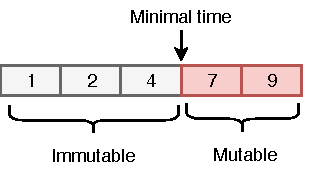
\includegraphics[width=.3\textwidth]{pics/immutable}
  \caption{Grouping bucket won't be modified up to element that corresponds to current minimal time}
  \label {immutable}
\end{figure}

\begin{figure}[htbp]
  \centering
  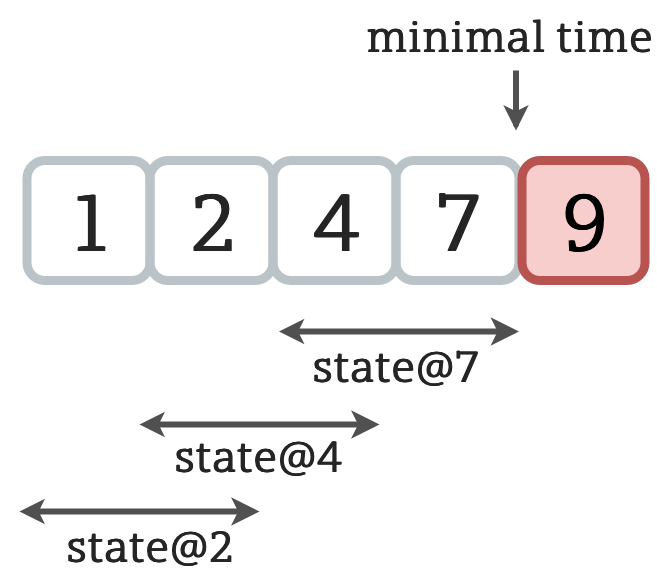
\includegraphics[width=.3\textwidth]{pics/substate}
  \caption{Grouping buckets with window = 2. Window-sized sublists are grouping states at past global times}
  \label {substate}
\end{figure}

Considering the properties mentioned above, the protocol of state snapshotting is the following:

\begin{itemize}
    \item On minimal time event, acker sends a request for the new snapshot along with minimal time notification
    \item When grouping operation receives the request, it asynchronously saves the state and sends back the acceptance message. The local state can be cleared after saving
    \item When barrier receives the request, it waits until producer acknowledges all in-flight bundles, and then sends back the acceptance message to the acker
    \item When acker receives all acceptance messages, it saves the global time of the snapshot to cluster state manager (ZooKeeper) 
\end{itemize}

This protocol is shown in Algorithm~\ref{state-snapshoting}.

\begin{algorithm}
\caption{State Snapshotting}
\label{state-snapshoting}
  \begin{algorithmic}
    \Process {Acker}
      \State $vertices \gets$ all physical groupings and barrier instances
      \State $snapshotted \gets \varnothing$
      \State $ongoingSnapshot \gets nil$
      \State
      \Event{$\langle MinTime, t \rangle$}
        \If {$ongoingSnapshot = nil$} \Comment{There is no unfinished snapshot}
          \For{{\bf all $v$} $\in vertices$}
            \State \Call{Send}{$v, \langle MinTime_{snap}, t\rangle$}
          \EndFor
          \State $ongoingSnapshot \gets t$
        \EndIf
      \EndEvent
      \Event{$\langle Snapshotted, v\rangle$}
        \State $snapshotted \gets snapshotted \cup v$
        \If {$snapshotted = vertices$}
          \State \Call{Save}{$ongoingSnapshot$} \Comment{Save time to cluster state manager}
          \State $snapshotted \gets \varnothing$
          \State $ongoingSnapshot = nil$
        \EndIf
      \EndEvent
    \EndProcess

    \Process {Grouping}
      \State $bucket[]$ \Comment{List of data items ordered by time}
      \State
      \Event{$\langle MinTime_{snap}, t\rangle$}
        \State \Call{Save}{t, bucket[0, t]} \Comment{Save substate to persistent storage}
        \State \Call{ClearRange}{bucket, 0, t}
        \State \Call{Send}{$acker, \langle Snapshotted, self\rangle$}
      \EndEvent
    \EndProcess

    \Process {Barrier}
      \State $lastAcknowledgedTime \gets -\infty$ \Comment{Time of the last acknowledged bundle by consumer}
      \State $postponedSnapshotTime \gets \infty$
      \State
      \Event{$\langle MinTime_{snap}, t\rangle$}
        \If{$lastAcknowledgedTime \geq t$}
          \State \Call{Send}{$acker, \langle Snapshotted, self\rangle$}
        \Else
          \State $postponedSnapshotTime \gets t$
        \EndIf
      \EndEvent
      \Event{$\langle Ack, t\rangle$}
        \State $lastAcknowledgedTime \gets t$
        \If {$postponedSnapshotTime < lastAcknowledgedTime$}
          \State \Call{Send}{$acker, \langle Snapshotted, self\rangle$}
          \State $postponedSnapshotTime \gets \infty$
        \EndIf
      \EndEvent
    \EndProcess
  \end{algorithmic}
\end{algorithm}

Acker can send requests for the new snapshot not for each minimal time event, e.g., it can skip request if the elapsed time since the last snapshot is less than some threshold. Parameters that influence the frequency of snapshots are in user's scope.

It is worth to note that any persistent key-value storage can be used as a storage for the state. Hash unit of the corresponding grouping operation concatenated with received minimal time can be used as a key. Waiting until barrier sends out all in-flight bundles is the only dependency between state snapshotting and barrier flushing mechanisms, that does not practically influence end-to-end processing latency. 

This protocol satisfies the following properties regarding the global time $GT$ that is written to cluster state manager:
\begin{enumerate}
    \item All stateful operations can restore the state that is reached after consuming all data items with global times in range $[0..GT)$ 
    \item All bundles that contain items with global times in range $[0..GT)$ have been already acknowledged by data consumer 
\end{enumerate}

Hence, this global time can be used as a resuming point after recovery without loss of consistency.

\subsection{Failure detection and recovery}
Typically, distributed systems take into consideration the following types of failures:
\begin{itemize}
    \item Packet loss
    \item Node failure
    \item Network partitioning
\end{itemize}

Network partitioning is the special case of failure because in this case computations cannot be restarted. We believe that in this case, stream processing does not make sense. To the best of our knowledge, there are no open-source stream processing systems that tolerate network partitioning.

As it was described above, acker traces data items using the table of XORs grouped by global time. Therefore, packet loss can be determined by the acker because the corresponding value in acker's table will not be nullified. Node failure can also be observed by the acker through periodical heartbeats. 

In case of packet loss or node failure, acker restarts the computations from the last successful checkpoint. The failure of the acker itself can be detected by cluster state manager, that triggers the same restart protocol. Restart protocol includes the following steps:

\begin{itemize}
    \item Acker reads the global time of the last snapshot from cluster state manager. After that, it broadcasts this global time to all grouping operations
    \item Grouping operations fetch their states from state storage using the corresponding hash unit and received global time as a key. After that, grouping operations send an acknowledgment that they are ready for processing to the acker 
    \item Barriers request the last released bundle from data consumers and send an acknowledgements that they are ready for processing to the acker
    \item When acker receives all acknowledgments from groupings and barriers, it requests data producer to replay starting from the global time of the last snapshot  
\end{itemize}

Proposed protocol guarantees the following properties:

\begin{itemize}
    \item Processing does not restart until all grouping operations obtain consistent states. The consistency of these states is guaranteed by the state snapshotting protocol
    \item Duplicates are not produced because, at the moment when processing is restarted, it is ensured that barrier has obtained the last released global time and is able to filter out extra items
    \item The last released global time cannot be less than the global time of the last snapshot. Therefore, data cannot be lost. This property is guaranteed in conjunction with the state snapshotting protocol
\end{itemize}

Therefore, the proposed protocol can be used for system restart without loss of exactly once semantics. Regarding at least once semantics, all protocol actions are the same, except waiting until the barriers are ready.
